\icode{N-ME-SI-L3-260627-001}
如图所示，一小物块被夹子夹紧，夹子通过轻绳悬挂在小环上，小环套在水平光滑细杆上，物块质量为\(M\)，到小环的距离为\(L\)，其两侧面与夹子间的最大静摩擦力均为\(F\)。小环和物块以速度\(v\)向右匀速运动，小环碰到杆上的钉子\(P\)后立刻停止，物块向上摆动。整个过程中，物块在夹子中没有滑动。小环和夹子的质量均不计，重力加速度为\(g\)。下列说法正确的是\paren[]
      
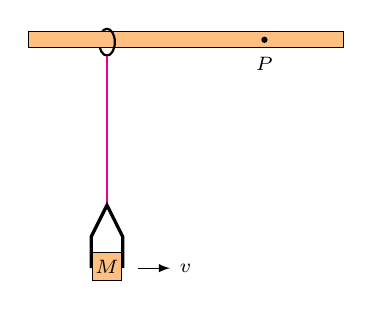
\begin{tikzpicture}[font=\scriptsize]
    \draw[thick] (0,.9) arc (-90:-270:.1 and .17);
    \draw[fill=orange!50] (-1,1.0)rectangle(3,1.2);
    \draw[thick] (0,.9) arc (-90:90:.1 and .17);
    \fill (2,1.1) circle(.04);
    \draw[magenta] (0,.9)--(0,-1);
    \draw[very thick] (-.2,-1.8)--(-.2,-1.4)--(0,-1)--(.2,-1.4)--(.2,-1.8);
    \draw[fill=orange!50] (-.18,-1.6) rectangle (.18,-1.96)node[pos=.5]{\(M\)};
    \draw[-latex] (.4,-1.8)--(.8,-1.8)node[right]{\(v\)};
    \node at(2,1)[below]{\(P\)};
\end{tikzpicture}
\begin{choices}
    \item 物块向右匀速运动时，绳中的张力等于\(2F\)
    \item 小环碰到钉子\(P\)时，绳中的张力大于\(2F\)
    \item 物块上升的最大高度为\(\frac{2v^2}{g}\)
    \item 速度\(v\)不能超过\(\sqrt{\frac{(2F - Mg)L}{M}}\)
\end{choices}
\begin{answer}
    D\qquad 提示：刚碰到\(P\)时，静摩擦力提供向心力，\(2F - Mg = M \frac{v^2}{L}\)
\end{answer}